\newsavebox\lstbox
\begin{lrbox}{\lstbox}
    \begin{minipage}{0.2\textwidth}
        \begin{lstlisting}[style=xmlfig]
<carte>
 <prix>10 euros</prix>
 <editeur> MICHELIN <editeur>
 <edition>2016</edition>
 <langue>Francais</langue>

  ...
</carte>\end{lstlisting}
    \end{minipage}
\end{lrbox}
\begin{tikzpicture}[]
    \node (xml) at (-3.6, -1.4) {\usebox\lstbox};
    \node[align=center,below] at (xml.south) {Modèle};

    % local bounding box to give a name to the pic: http://tex.stackexchange.com/a/241737/32098
    \pic[local bounding box=carte] (carte) at (0, 0) {france={scale 0.15}};
    \node[align=center,below] at (carte.south) {Modèle};

    \node[inner sep=2pt] (photo) at (6,-1.4) {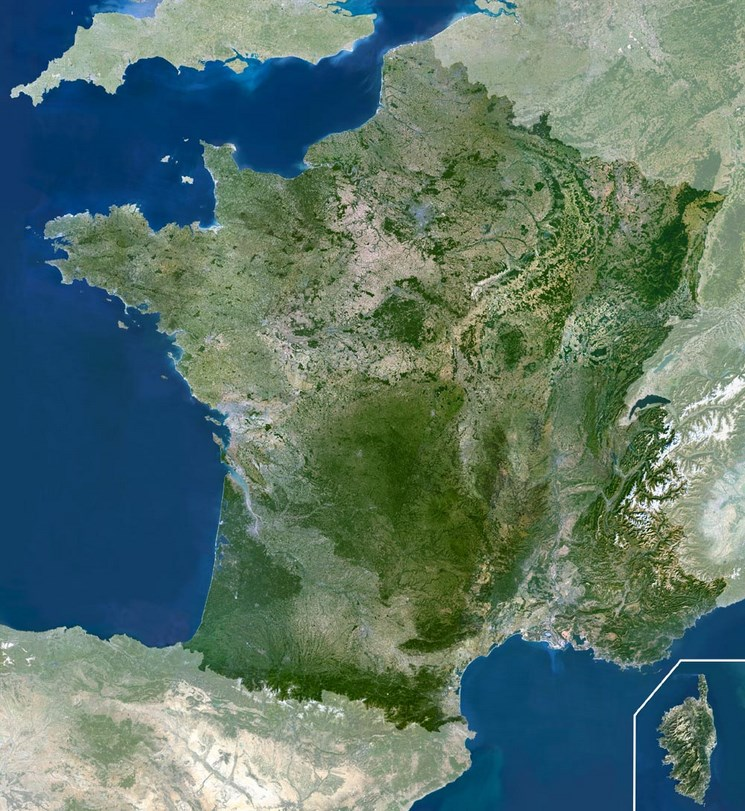
\includegraphics[scale=0.09]{figures/lib/france_satellite.jpg}};
    \node[align=center,below] at (photo.south) {Système modélisé};

    % fleches
    \draw[->] (carte) -- (photo.west) node[midway,above] {Représente} node[midway,below]{$\mu$};
    \draw[->] (xml) -- (carte.west) node[midway,above] {Représente} node[midway,below]{$\mu$};
\end{tikzpicture}
